\documentclass[12pt]{../notes}

% Command for Questions
%\question{}

% Command for Notes
% \note{}

% Code to create a minipage where you can type in class notes. 
%%\begin{minipage}[l][2cm][c]{\textwidth}
%\begin{comment}

%\end{comment}
%%\end{minipage}


% Begin Document
%==============================================================================
\begin{document}
% Include the Title of the Handout
\ntitle{5.1: Logistic Regression}

% Include Numbered Sections
\section{Why Logistic Regression?}

Recall the example from 5.1.1 where we try to predict the odds of having a disease using:
\begin{itemize}
\item Age (in years)
\item Sector (1 if living in high risk city sector, 0 otherwise)
\end{itemize}

\question{Based on the output in Figure \ref{fig:logit_output} what is the \textit{probability} that a 40 year old living in the high risk city sector has the disease?}

\begin{minipage}[l][5cm][c]{\textwidth}
%\begin{comment}
\note{$$\hat{L} = -2.335 + 0.0293*40 + 1.6734*1 = 0.5104$$}

\note{$$\hat{\pi} = \frac{1}{1 + e^{-0.5104}} = 0.6249$$}

\note{There is a 62.49\% chance.}
%\end{comment}
\end{minipage}

\nspace
\question{Using the same information provided in Figure \ref{fig:logit_output}, provide an interpretation of the coefficient associated with Age?}

\begin{minipage}[l][5cm][c]{\textwidth}
%\begin{comment}
\note{Holding city sector constant, a one year increase in age multiplies the odds of having the disease by $e^{0.0293} = 1.0297$}

\nspace
\note{Holding city sector constant, the odds of having the disease are $100(e^{0.0293} - 1) = 2.97\%$ greater for each year increase in Age.}
%\end{comment}
\end{minipage}




\begin{figure}[H]
\centering
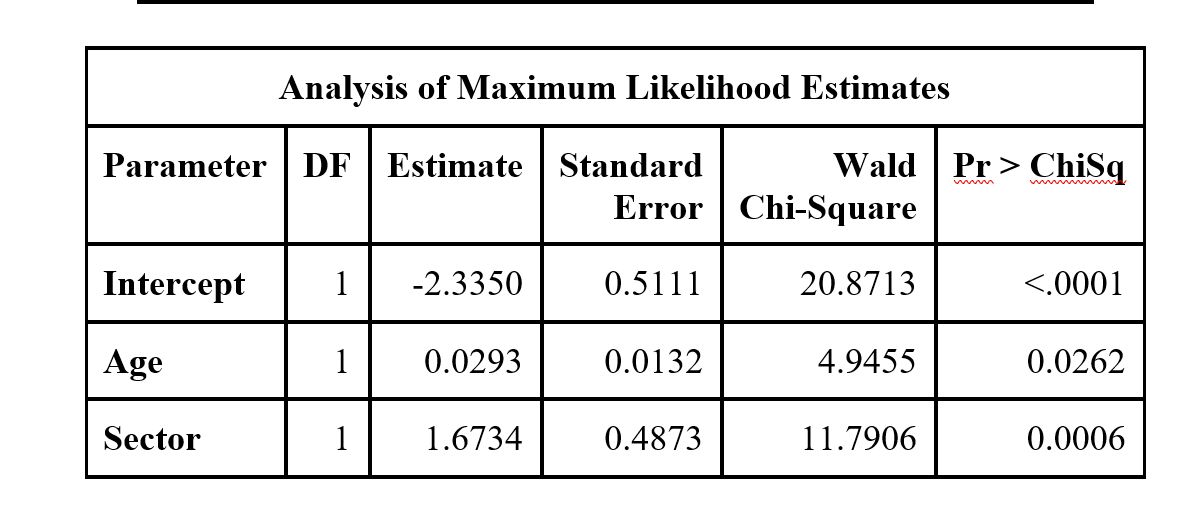
\includegraphics[width = 0.75\textwidth]{../figures/module5/logit_output_sample.png}
\caption{Sample logistic regression output.}
\label{fig:logit_output}
\end{figure}

\nspace

\question{Can you think of an example where we might want to make the probability threshold for predicting a ``1'' be less than 0.5?}

\begin{minipage}[l][4cm][c]{\textwidth}
%\begin{comment}
\note{Any example where the consequence of a false positive (predicting one when the answer is in fact zero) is much less costly than a false negative (predicting 0 when the answer is in fact 1).} 

\nspace
\note{Example, predicting someone has COVID-19 given demographic variables. It may be useful to make threshold for a 1 prediction less than 50\% because it is less costly to quarantine someone who is not actually infected than it is to not quarantine someone who is infected.}
%\end{comment}
\end{minipage}

\question{Using non-technical terms, how might you describe an outlier in logistic regression?}

\begin{minipage}[l][3cm][c]{\textwidth}
%\begin{comment}
\note{Observing a positive (or negative) result when the chance of observing a positive (or negative) result is extremely low. }
%\end{comment}
\end{minipage}



% End the Document
%==============================================================================
\end{document}